\documentclass{acm_proc_article-sp}
\usepackage{fancyhdr}
\usepackage{amssymb}
\usepackage{amsmath}
\usepackage{amsfonts}
\usepackage[T1]{fontenc} % get tt fonts to work right
\usepackage{graphicx}
\usepackage{fixltx2e}
\usepackage{multirow}
\usepackage{color}
\usepackage{caption}
\DeclareCaptionType{copyrightbox} % workaround for bug in caption
\usepackage{subcaption}
\usepackage{xspace}
\usepackage{url}
\usepackage{listings}

\begin{document}

\special{papersize=8.5in,11in}
\setlength{\pdfpageheight}{\paperheight}
\setlength{\pdfpagewidth}{\paperwidth}

\definecolor{darkblue}{rgb}{0,0,0.7}
\definecolor{darkgreen}{rgb}{0,0.5,0}
\definecolor{orange}{rgb}{0.7,0.5,0.0}
\definecolor{brown}{rgb}{0.8,0.4,0.0}

\definecolor{teal}{rgb}{0.06,0.3,0.3}
\definecolor{maroon}{rgb}{0.5,0.0,0.25}
\definecolor{darkblue}{rgb}{0.0,0.2,0.75}
\definecolor{darkred}{rgb}{0.7,0.0,0.0}
\definecolor{darkgreen2}{rgb}{0,0.35,0}
\definecolor{darkgreen}{rgb}{0,0.5,0}
\newcommand{\timnote}[1]{ {\textcolor{maroon} { Tim: #1 }}}
\newcommand{\todo}[1]{ {\textcolor{red} { TODO: #1 }}}

\title{How low can you halo?}
\subtitle{Modeling halo exchange on multi-dimensional torus networks}

\numberofauthors{2}

\author{
% 1st. author
\alignauthor
Yadu Nand Babuji\titlenote{todo}\\
       \affaddr{Dept. of Computer Science,}\\
       \affaddr{University of Chicago,}\\
       \affaddr{Chicago, IL, USA}\\
       \email{yadunand@uchicago.edu}
% 2nd. author
\alignauthor
Timothy G. Armstrong\titlenote{todo}\\
       \affaddr{Dept. of Computer Science,}\\
       \affaddr{University of Chicago,}\\
       \affaddr{Chicago, IL, USA}\\
       \email{tga@uchicago.edu}
}
\maketitle

\begin{abstract}
% Motivation
Many High Performance Computing (HPC) applications involve application domain decompositions that involve nearest neighbor communication.
Halo exchange is a common nearest neighbor communication pattern used for solving PDE's and thus applying to a wide range of HPC applications.
% Problem statement % Approach
Empirical results show that different task placement strategies in Halo exchange codes can have as much as 7.5x performance difference.
We develop an analytical model to understand the impact of task placements withing a network topology on performance and guide selection of
optimal mappings.
% Results
Analytic model comes with x percentage of empirical results with a max error of E.
Identified optimal and pessimal mappings.
% Conclusions

\todo{Complete the Abstract}

\end{abstract}

\section{Introduction}

% Intro
Halo exchange is a common communication pattern in parallel codes, where
each process is assigned an application subdomain and must periodically
communicate with other processors that have neighboring subdomains to
update information about the state of the boundary between subdomains.
A common special case is when a multi-dimensional cartesian space is
decomposed into subdomains of equal size.  For example, in the three-dimensional
case, a 8x8x8 cube might be decomposed into 256 2x1x1 cubes for execution on 256 processors.

% Objective
This paper explores the problem of mapping such multi-dimensional cartesian
halo exchange communications onto parallel computers with hypercube or
torus networks. A typical computation job on a leadership class machine would
utilize several hundreds to thousands of cores, as a result there are a large number of
possible mappings to the physical hardware that could be chosen. We seek to understand
what aspects of the mappings have an impact on performance and how to quantify them so
that the impact these mappings have on performance can modelled. Mapping strategies
are a very cheap optimisation which requires no code changes to the application
and as our empirical studies show, these mapping stategies have significantly
different network performance characteristics. There are no studies to the best
of our knowledge that attempts to model the impact of mapping performance on
HPC systems.

% What does this paper contribute:
\todo{Add following points with text}\\
1. An analytical model that describes the perfomance on Halo exchange with different mappings\\
2. A nearly worst and optimal mapping.\\

The rest of the paper is organised as follows :
% Guidance
The rest of the paper is organised as follows: Section 2, provides background information on
the HPC system topologies and BlueGene/Q in particular. Section 3, describes mapping strategies.
Section 4, develops the analytical model and Section 5, details the experiment design for empirical
validation of the model.

% Summary conclusions

\section{High-Performance Computer Networks}

The state of the art in High Performance Computing(HPC) infrastructure, demands high-performance networks
to support the movement of data between the nodes as well as to-and-from disk-arrays. HPC systems are
increasingly architected with high radix interconnects such as hypercubes and N-dimensional tori.
Parallel applications have a wide range of task placements options to exploit the network topology of
these HPC systems. These networks have evolved to several different network topologies in order to support
different requirements, and data movement patterns. For HPC applications which involve fine-grained communication,
high-radix networks provide low latency, smaller diameter, and large bandwidth as multiple links along the multiple
dimensions supprted.

% Routing protocols on the BG/Q
% Direct routing
% Adaptive routing
\subsection{Blue Gene/Q 5D torus network}

The BlueGene/Q is a 3rd generation massively parallel supercomputer from IBM. The BlueGene/Q implements a 5 dimensional torus with up to 16K nodes.
To support the 5 dimensional torus each compute node has 10 bi-directional duplex links. There is a separate 11th link for IO. Each of the 10 links
operate at a bandwidth of 2GB/s \cite{BGQ_RedBook_2013}. After accounting for 10\% overhead in message headers 1.8GB/s is available for raw data per link in one-direction.
The 5D torus network provides high nearest neighbor bandwidth as well bisection bandwidth while decreasing the maximum number of hops to reach
the furthest nodes. The five dimensions on the network are labelled as
A,B,C,D,E.  The location of a compute node in a job can be specified
by its A,B,C,D,E coordinates, while the location of a core is specified
with an additional dimension, T. The E dimension is limited to a length
of 2, while A,B,C,D dimensions can be multiples of 4 to remain torus.
One rack on the BlueGene/Q is a torus network of dimensions 4x4x4x4x2.
Larger torus networks are formed by combining these 4x4x4x4x2 racks.
The intranode per hop latency is approximately 40ns BGQ \cite{BGQ_Interconnect_2012}, 
while the worst point-to-point network latency is expected to be under 3$\mu$s. 

% The BGQ routing protocols
The BlueGene/Q implements two routing protocols for point-to-point communication.
Deterministic routing is designed for small messages, where packets sent between two nodes always follow the same direct path.
This routing method is simple and has overhead but can result in hotspots
when traffic between several nodes cross on some node.
Adaptive routing determines the route for packets at the runtime taking current network loads into consideration.
This routing mechanism balances the network load for a penalty in latency.


\subsection{Message Passing Interface(MPI)}
The Message Passing Interface (MPI) is a standard for message-passing in HPC applications.
We use MPI to implement the messaging and synchronization aspects of the HALO exchange code,
and hence the performance observed from running the application would be influenced by the behavior of MPI due to its various protocols on the BlueGene/Q.
There are four protocols supported by the MPI implementation used BlueGene/Q.
The protocol utilized by MPI is determined by the size of the message that is being sent.  The short and immediate protocols are used for very short
messages that can fit in a single network packet.  The rendezvous
protocol is used for longer messages where receiver buffer space may
be insufficient to store the message and where more complex adaptive
routing protocols may be beneficial.  The eager protocol
is used for medium length messages that require multiple packets,
but where the overhead of the rendezvous protocol outweighs any
benefits.
The data sizes at which the switch to different protocol occurs is configurable, but for our experiments we use the defaults on BlueGene/Q, which are 
listed in Table~\ref{table:bgq_protocols}.

% Add note on : Intranode latency implemented as in-memory copy
% Large message copies as RDMA copy.
MPICH2 Nemesis.

\begin{table}
  \caption{MPI Protocol default thresholds
    \label{table:bgq_protocols}}
  {\footnotesize
    \begin{tabular}{ | l | l | l | p{1.5cm} |}
    \hline
    Protocol   & Min Msg Size   & Max Msg Size  & Routing\\ \hline
    Immediate  &             0B &           112B & Direct\\ \hline
    Short      &           113B &           496B & Direct\\ \hline
    Eager      &           497B &          4096B & Direct\\ \hline
    Rendezvous &          4096B &      unlimited & Adaptive\\ \hline
    \hline
    \end{tabular}
  }
\end{table}

\section{Mapping Strategies}\label{sect:mapping}
Different classes of HPC systems provide different mechanisms and varying levels of control on task placement.
The MPI framework gives finegrained control of placement of tasks via a mapping file when such functionality
is supported by the hardware. On BlueGene/Q systems from IBM, the mapping files allow you to determine where
each MPI rank is placed within a machine partition. On Cray XE6 machines, which do not have the notion of
isolated machine partitions, the mapping functionalities only give the flexibility of choosing the node on
which a set of ranks will execute on, but not the physical proximity of the nodes with relation to each other.
The Cray XE6 does not guarantee isolation of the network from the traffic generated by other users and it
also cannot guarantee that the location of nodes with relation to the rest of the nodes would remain constant
across multiple runs. As a result BlueGene/Q systems can offer far greater control on task placements, and
better guarantees on reproducible results.

The BlueGene/Q mapping file follows a simple text format, with one
line per MPI rank.  The $i$th line in the file gives the A,B,C,D,E,T
coordinates of MPI rank $i$ as space-separated integers.

With the focus on BlueGene/Q systems we will outline a range of different mapping strategies we have examined.

\subsection{Regular/Default Mapping}
The default mapping involves ranks being assigned in increasing order along the dimensions T, E, D, C, B, A.
Assuming that we assign 16 ranks with one rank per core, the first 16 ranks from the application domain will
be on the node with address (0 0 0 0 0) and so on. Since the ranks in the application domain are assigned in
some increasing order, nodes along a particular dimension will be grouped on each node. This mapping works
very well when the dimensionality of the application domain and that of the partition match. For eg, if the
application domain were 4x4x4x4x2 and we were running one rank per node, there is a one to one mapping to the
network where this mapping would retain nearness between all neighbors. However when the length of dimensions
in the application domain and network or the dimensionality do not match, this mapping scheme will not perform as well.

Sample from the mapping file :
\begin{lstlisting}[frame=lines, basicstyle=\ttfamily,columns=fixed]
0 0 0 0 0 0
    ...
0 0 0 0 0 15
0 0 0 0 1 0
    ...
0 0 0 0 1 15
0 0 0 1 1 0
    ...
0 0 0 1 1 15
\end{lstlisting}

\subsection{Linear Mapping}
Linear mapping refers to placing ranks along nodes in the increasing order of dimensions A, B, C, D, E, T.
As a result the neighboring ranks in the application domain along a dimension are places on nodes atleast
one hop away.

Sample from the mapping file :
\begin{lstlisting}[frame=lines, basicstyle=\ttfamily,columns=fixed]
0 0 0 0 0 0
1 0 0 0 0 0
2 0 0 0 0 0
3 0 0 0 0 0
0 1 0 0 0 0
1 1 0 0 0 0
2 1 0 0 0 0
3 1 0 0 0 0
0 2 0 0 0 0
\end{lstlisting}

\subsection{Skewed Mapping}

Skewed mapping uses a modified order of task placement along a dimension.
With linear mapping the nearest neighbors along, say dimension A are only one hop away along A+ or A-.
Skewed mapping uses an alternate ordering on task placement to ensure that one of the neighbors is atleast
2 hops away. This alternate ordering is shown in Fig. \ref{fig:Skewed layout for 4 Nodes in 1D}.
Since the network is torus, the maximum distance possible along any dimension is the length along
the dimension divided by two. However, since there are 5 dimensions on a Blue Gene/Q creating a skew along different
dimensions can create mappings in which the nearest neighbors are not only separated by hops along a dimension but
along different dimensions. Skewed mappings can be generated by introducing skew along the order of dimensions
A,B,C,D,E,T or along the reverse order. The regular ordering places the neighbors on the same node while the reversed
ordering places each rank on different nodes in the skewed ordering.

Sample from the mapping for regular ordering:
\begin{lstlisting}[frame=lines, basicstyle=\ttfamily,columns=fixed]
0 0 0 0 0 0
  ...
0 0 0 0 0 15
0 0 0 0 1 0
  ...
0 0 0 0 1 15
0 0 0 2 0 0
  ...
0 0 0 2 0 15
\end{lstlisting}

Sample from the mapping for reversed ordering:
\begin{lstlisting}[frame=lines, basicstyle=\ttfamily,columns=fixed]
0 0 0 0 0 0
2 0 0 0 0 0
1 0 0 0 0 0
3 0 0 0 0 0
0 2 0 0 0 0
2 2 0 0 0 0
1 2 0 0 0 0
3 2 0 0 0 0
\end{lstlisting}


\label{sect:Skewed mapping in 1D}
\begin{figure}
  \center
  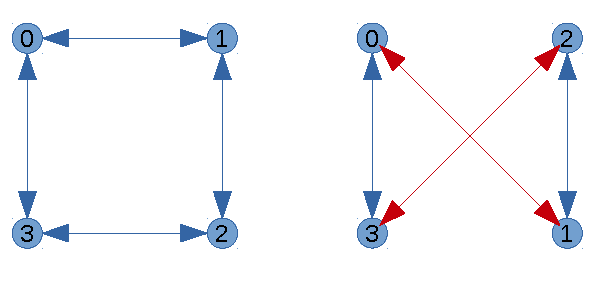
\includegraphics[width=0.475\textwidth]{skewed_layout_cropped.pdf}
  \caption{Skewed layout for 4 Nodes in 1D}
    \label{fig:Skewed layout for 4 Nodes in 1D}
\end{figure}

\subsection{Random Mapping}
\label{sect:random}

Random mappings are generated by using the linux shuf utility to shuffle the mapping file from regular mapping.
Since the mappings are random we would expect the average distance between nodes to be close to half the diameter
or the maximum distance between any two nodes in the network. The random mappings generated for a partition of
dimensions 4x4x4x4x2 with 16 ranks per node have an average distance of 4.0035 \todo{Update with corrected average distance}.
The diameter of network is the sum of the halves of the length of each dimension : 9.


\subsection{Deoptimized Mappings from Simulated Annealing}
In order to cover an even wider range of mappings, we tried to
devise mappings that were worse than the random mapping.
We can obtain an absolute upper bound on average distance of
$9$, because the maximum possible distance in a 5D torus
partition of 4x4x4x4x2 is 9.  It is unclear to us whether
mappings with average distance of $9$ exist, and under what
circumstances they might exist: we were unsuccessful in
attempts to reduce this upper bound.  We were also
unsuccessful in directly devising mappings
with average distance significantly greater than the $~4.5$ average
distance obtained with random mapping.

In order to discover mappings with high average distance, we used
a heuristic optimization algorithm that began with a random mapping
and made incremental modifications in an attempt to discover mappings
with higher average distance.
We selected to use simulated annealing~\cite{Press2007} because of the
simplicity and effectiveness of this family of heuristics.

A simulated annealing optimization run starts with aggressive exploration
of the search space, where large perturbations are made and negative
moves are sometimes accepted to allow the algorithm to escape local
minima of the function being optimized.  Over time, the algorithm
transitions to fine-tuning, with smaller perturbations made and negative moves
accepted less frequently.  Pseudocode for the algorithm is shown in
Figure~\ref{fig:anneal_pseudocode}.

\begin{figure}
  {\footnotesize
  \begin{lstlisting}[frame=lines, basicstyle=\ttfamily,columns=fixed]
mapping := random_mapping(app_topo, net_topo)
dist := average_distance(mapping)
for i = 1 to niters do
  temp := calc_temp(i, niters)
  nswaps := calc_swaps(temp, nranks)
  new_mapping := random_swap(mapping, nswaps)
  new_dist := avg_dist(new_mapping)
  if new_dist > dist or
     accept(dist, new_dist, temp) then
    mapping := new_mapping
    dist := new_dist
  end
end
  \end{lstlisting}
  }
  \caption{Pseudocode halo exchange algorithm with concurrent sends and
           receives to all neighbours.}
    \label{fig:anneal_pseudocode}
\end{figure}

The algorithm has several inputs and has several subprocedures,
which we will describe informally.
\texttt{niters} is the number of annealing iterations to attempt, while
\texttt{app\_topo} and \texttt{net\_topo} are data structures
describing the application and network topology, respectively.

\texttt{random\_mapping} initializes a random mapping, as described
in Section~\ref{sect:random} using the topology information.
\texttt{avg\_dist} computes the average distance between
application neighbors (i.e. ranks that exchange messages in
halo exchange) for the mapping.

\texttt{random\_swap} randomly selects \texttt{nswaps} pairs of ranks
and swaps them, with \texttt  The \texttt{calc\_swaps} function computes
the number of ranks to swap up to 2\% of ranks, swapping more at higher
temperatures:
$$calc\_swaps(temp, nranks) = max(1, \lfloor 0.02 * temp * nranks \rfloor)$$

The \texttt{calc\_temp} function returns a temperature that
decreases from 1 to 0 during the course of the annealing process.
The basic trajectory followed is cubic decrease: $(1 - i/niters)^3$.
Additional cycles of raising and lowering the temperature are also
applied to diverge from this basic trajectory.

\texttt{accept} decides whether to accept a mapping that has lower
average distance, which can the algorithm escape a local maximum.
This is randomized based on a random value $p$ between 0 and 1.
The new mapping is accepted if:
$$temp * (0.5 - (1.0 - new\_dist/dist) * 25) > p$$

Using this approach for upwards of 1 million iterations,
we were able to produce mappings that had average distance substantially
higher than the randomized mapping, although still short of our upper
bound of $9$.  We obtained...  \timnote{Yadu - fill in numbers}

\subsection{Topology aware box partitioned Mapping}

The box partitioned mapping is designed with the goal of placing N-dimensional slices of the application domain on nodes such that
intranode halo messaging is maximised. This should in-turn reduce network traffic and increase overall performance.
We break down the application domain to multi-dimensional slices and place them on adjacent nodes in the network so that that the
overall distance the traffic that exits the node has to travel is minimised. The size and dimensionality of the box is informed
by the network topology and the application domain.

For an application with a 3D domain decomposition of 32x32x8, the box is determined to be 4x2x2. We partition the application domain
into 512 contiguous 3D slices of dimensions 4x2x2. Now, there are 512 boxes arranged as 8x16x4 (32x32x8/4x2x2).
The 512 slices are then mapped on to the 4x4x4x4x2 network topology of the BlueGene/Q.

Sample from the mapping for 3D application of dimensions 32x32x8 to network of dimension 4x4x4x4x2x16
\begin{lstlisting}
0 0 0 0 0 0
0 0 0 0 0 1
0 0 1 0 0 0
0 0 1 0 0 1
0 0 2 0 0 0
0 0 2 0 0 1
0 0 3 0 0 0
0 0 3 0 0 1
\end{lstlisting}

For an application with a 5D domain decomposition of 8x8x8x8x2, the box is determined to be 2x2x2x2. Similar to the 3D case, we
partition the application domain into 512 contiguous into  slices of dimensions 2x2x2x2.
Now, there are 512 boxes arranged as 4x4x4x4x2 (8x8x8x8x2/2x2x2x2). There is a simple one to one mapping from the
to that of the 4x4x4x4x2 network topology since the dimentionality matches exactly. The difference between the mapping
generated by this method and the regular mapping stems from the mismatch of dimensions in the application domain to that
of the network topology.

Sample from the mapping for 5D application of dimensions 8x8x8x8x2 to network of dimension 4x4x4x4x2x16
\begin{lstlisting}
0 0 0 0 0 0
0 0 0 0 1 0
0 0 0 0 0 1
0 0 0 0 1 1
0 0 0 1 0 0
0 0 0 1 1 0
0 0 0 1 0 1
0 0 0 1 1 1
\end{lstlisting}

\subsection{Metrics for measuring a mapping}

In the earlier sections we have introduced several different mapping strategies, each with different characteristics which could
impact the network performance. To relate the impact of a mapping on network performance it is important to device a metric that
captures the aspects of a mapping that could affect the network. Mappings determine the amount of intranode communication versus
the communication that must go over the network, and over what links these communication occurs.

While a direct path with the manhattan distance between neighbors would be chosen when message sizes are small and deterministic routing
protocol are in place, more interesting network effect become apparent only when message sizes increase. Once message sizes exceed 4Kb
rendezvous protocol is used by the network which involves complex routing logic to avoid hotspots, and increase network utilization for
a penalty in latency. Since it is difficult to model these dynamic systems, we will assume that the rendezvous protocol will balance
the network load evenly such that the messages flowing over every link is similar.


The average distance between neighbors can easily be calculated by taking the average of the manhattan distance of all pairs of neighbors.
We assume that the distance between two ranks on the same node is 0, since intranode messaging does not contribute to network traffic.
This average distance \textbf{N\textsubscript{steps}}, can now be treated as a proxy for average network traffic flowing over any particular 



Let the torus network be of \textbf{D} dimensions, and let \textbf{N\textsubscript{ranks}} be the number of ranks in the partition.
The total logical neighbors involved in halo exchange is :
\begin{equation}
  T_{neighbors} = N_{ranks} * 2 * D
\end{equation}

Consider every pair of neighbor nodes (u,v), the manhattan distance between nodes u,v is calculated by the distance function \textbf{dist\textsubscript{(u,v)}}.
The average number of messages flowing through any link is given by:

\begin{equation}
  N_{steps} = \frac{ \sum\limits_{u,v} dist_{u,v} } {T_neighbors}
\end{equation}

The average distance for the various mappings for the 3D and 5D case are provided in table


\begin{table}
  \caption{Average distance for mappings from 8x8x8x8x2 domain to 4x4x4x4x2x16 topology}
  {\footnotesize
    \begin{tabular}{| l | l | p{1.5cm} |}
    \hline
    Mapping         & Avg. Distance & Max Dist\\ \hline
    regular         & 1.050000 & 3.000000\\ \hline
    linear          & 1.450000 & 3.000000\\ \hline
    reversed        & 1.450000 & 3.000000\\ \hline
    random          & 4.504980 & 9.000000\\ \hline
    skewed regular  & 1.100000 & 3.000000\\ \hline
    skewed reversed & 1.450000 & 3.000000\\ \hline
    optimal         & 0.600000 & 1.000000\\ \hline
    de-optimized    & --       & --      \\ \hline
    \hline
    \end{tabular}
  }
\end{table}


\begin{table}
  \caption{Average distance for mappings from 32x32x8 domain to 4x4x4x4x2x16 topology}
  {\footnotesize
    \begin{tabular}{| l | l | p{1.5cm} |}
    \hline
    Mapping         & Avg. Distance & Max Dist\\ \hline
    regular         & 1.145833 & 4.000000\\ \hline
    linear          & 1.625000 & 4.000000\\ \hline
    reversed        & 1.625000 & 4.000000\\ \hline
    random          & 4.499023 & 9.000000\\ \hline
    skewed regular  & 0.979167 & 4.000000\\ \hline
    skewed reversed & 1.645833 & 4.000000\\ \hline
    optimal         & 0.479167 & 2.000000\\ \hline
    de-optimized    & 6.530436 & 9.000000\\ \hline
    \hline
    \end{tabular}
  }
\end{table}


\section{Analytical Model for Network Communication}\label{sect:model}

\timnote{Maybe this discussion should be moved further down -
it mainly pertains to $t_b$?  Do we also need to discuss the startup
time/different protocols here?}

There are a wide range of possible models that could be used to
estimate network communication performance for a complex network
such as those on BlueGene/Q or Cray XE6.  These models range from
full-fidelity simulations that directly simulate packet routing, to
simplified models that estimate performance based on simplifying
assumptions.  These simplified models are often very useful for
understanding and prediction, but typically have a limited domain
of applicability.  For example, network models that ignore congestion
can be suitable for modeling single point-to-point transfers, but are
unsuitable for modeling many simultaneous transfers over a shared network.

For halo exchange, we need a model that captures multiple
simultaneous data transfers contending for shared resources: we
expect that many of these messages will need to transit the
same network links.  We can, however, simplify the model by exploiting the
symmetry of the communication pattern, in which each MPI rank sends
and receives the same amount of data. For this reason, we chose to
use a model that assumes that traffic is distributed fairly evenly
throughout the network and that communication throughput is limited
by the aggregate capacity of the network's links. 

We arrived at our model for \textbf{t\textsubscript{b}} based on two assumptions.
We first assume that the limiting factor on transfer throughput will be
the most trafficked link on the network - the one that the most bytes
must transit during the halo exchange.  Finding the most trafficked
link and determining the number of bytes transferred is not feasible for our
simple model, because it would require simulating network load and
the Blue Gene/Q adaptive routing algorithms. We make a second assumption
that traffic is distributed fairly evenly across the network because of
the halo exchange pattern and adaptive routing, the maximum number of bytes
transiting a link will be closely correlated with the average number of bytes transiting a link.

On an HPC system such as BlueGene/Q or Cray XE6, each node has multiple duplex links to it's neighbors.
If the application on every node attempts to exchange messages with every neighbor, we can assume that
every link on the network will see similar traffic. Thus we, consider a single link and it's bandwidth
to determine \textbf{t\textsubscript{b}} the time required to send a Byte along the link.
Assume that there are \textbf{N\textsubscript{procs}} number of identical processes all of which will attempt to utilize the same links.
To capture the differences between different mappings we use a simple program to calculare the average distance between neighbors,
\textbf{N\textsubscript{steps}}. The current MPI implementation on leadership class systems like Mira (Bluegene/Q) utilizes
shared memory for intranode communication. When a neighbor is present within the same node, the link
is weighted as zero, and every network link or hop is weighted as one. Since it is possible to place
neighboring tasks from the application domain on the same node there are mappings possible which
minimize N\textsubscript{steps} below one. There are constant costs involved in startup, acquiring a buffer etc,
and t\textsubscript{c} is an experimentally calibrated constant that is a catch-all for the various constant costs
of network communication using MPI. N is the message size in bytes that are exchanged between neighbors.

The network load balancing provided by the rendezvous protocol comes with an added cost, which has to be
accounted for from experimental data. The memory reads, cache misses that occur as the message buffers exceed
the sizes of the caches etc are not accounted for. We will use an experimentally calibrated constant \textbf{$\alpha$}
which will represent the additional costs of messaging that has not been taken into account in the model.

A simple analytical model determines the time to completion, T of a complete halo exchange operation,
from the variables defined above as follows:
\begin{equation}
  T = t_c + (N_{steps} * N_{procs} * N * t_b * \alpha)
\end{equation}


\section{Experimental Design}\label{sect:experimental design}

Empirical studies are necessary to gauge the effectiveness validity of models. Considerable efforts have
been taken to ensure that the experiments are fair and are an accurate reproduction of the Halo exchange pattern
in real world scenarios. The experiments have been repeated multiple time on different partitions on the machine
to ensure that partition specific effects do not influence results, however we have not been able to reproduce
results on different machines of the same architecture due to time limitations.

\begin{figure*}[HT]
  {\footnotesize
  \begin{lstlisting}[frame=lines, basicstyle=\ttfamily,columns=fixed]
MPI_Comm comm_cart
MPI_Request req[4*N_dims]

for dim = 1 to N_dims do:
    MPI_Cart_Shift (comm_cart, dim,  1, rank_src[0][dim], rank_dst[0][dim]
    MPI_Cart_Shift (comm_cart, dim, -1, rank_src[1][dim], rank_dst[1][dim]
end

MPI_Barrier(comm_cart)
halo_timer(begin)
for dim = 1 to N_dims do
    # Send/recv message along dim+
    MPI_Isend(send_buffer, datalength, destination_ranks[0][dim], comm_cart, req[i*4])
    MPI_Irecv(send_buffer, datalength, source_ranks[0][dim], comm_cart, req[i*4+1])
    # Send/recv message along dim-
    MPI_Isend(send_buffer, datalength, destination_ranks[0][dim], comm_cart, req[i*4+2])
    MPI_Irecv(send_buffer, datalength, source_ranks[0][dim], comm_cart, req[i*4+3])
end

MPI_Waitall(4*N_dims, req)
MPI_Barrier(comm_cart)
halo_timer(end)
  \end{lstlisting}
  }
  \caption{Pseudocode halo exchange algorithm with concurrent sends and
           receives to all neighbours.}
    \label{fig:halo_pseudocode}
\end{figure*}

Since we are only interested in the network performance aspect of the halo exchange code, we only measure
the time taken to complete halo exchanges. The pseudocode for the halo exchange is listed in Figure~\ref{fig:halo_pseudocode}.

\subsection{Latency}
On the BlueGene/Q, the latency between the closest node and the farthest node is estimated to be under 3$\mu$s\cite{BGQ_Interconnect_2012}.
Since halo exchange is a collective operation, the entire operation is only as fast as the worst performer in the entire operation.
In the analytical model described in Section\ref{sect:model}, we assume that latency does not play a role.
This assumption is experimentally tested by comparing the time to completion of halo exchanged between the default mapping and a modified
mapping which has just two ranks interchanged to nodes that span the diameter of the torus. This results in the an increase in maximum distance
from 3.0 to 9.0 and increase of 0.003 for the average distance between neighbors.

\subsection{Cache effects}
To determine whether the network performance is affected by the send/receive message buffers overflowing from the
L3 caches, we designed an experiment which sent \textbf{DUPES} number of messages each with $\frac{datalength}{DUPES}$
message size. The runs were compared against a run with DUPES=1. The expected result is that for smaller datasizes
the time to completion will be higher when duplicate messages are sent as there is the added startup cost for \textbf{DUPES} times the original messages.
If the caches were indeed affecting the network performance, at higher data sizes, the Halo runs with duplicates should outperform
a run without duplicates.

\subsection{Task placement within Mappings for 3D and 5D application domains}
We've described eight different mapping schemes in Section \ref{sect:mapping}.
To study the network performance of the halo exchange codes, they are exercised using varying levels of data lengths for message exchanged between neighbors.
Multiples of 2 ranging from 8B to 32Mb,  are chosen as data sizes as they are representative of the various phases of MPI messaging protocols, and cover
a reasonable swath of datasizes that real world application might use. The hardware partitions chosen are 512 Node partitions of 4x4x4x4x2 shape. This
is one rack on the BlueGene/Q, and is comparable to partition sizes used by HPC applications.

The Halo exchange code itself measures the performance of various blocking and non-blocking MPI send and recv primitives and combinations.
For our experiments we will only consider MPI\_Isend and MPI\_Irecv primitives with no artificial delay introduced after the barrier.
The pseudocode for the halo exchange is listed here \ref{fig:halo_pseudocode}.
Evaluating the performance of the different MPI primitives with randomised delay options is beyond the scope of this paper.

\begin{figure}
  \center
  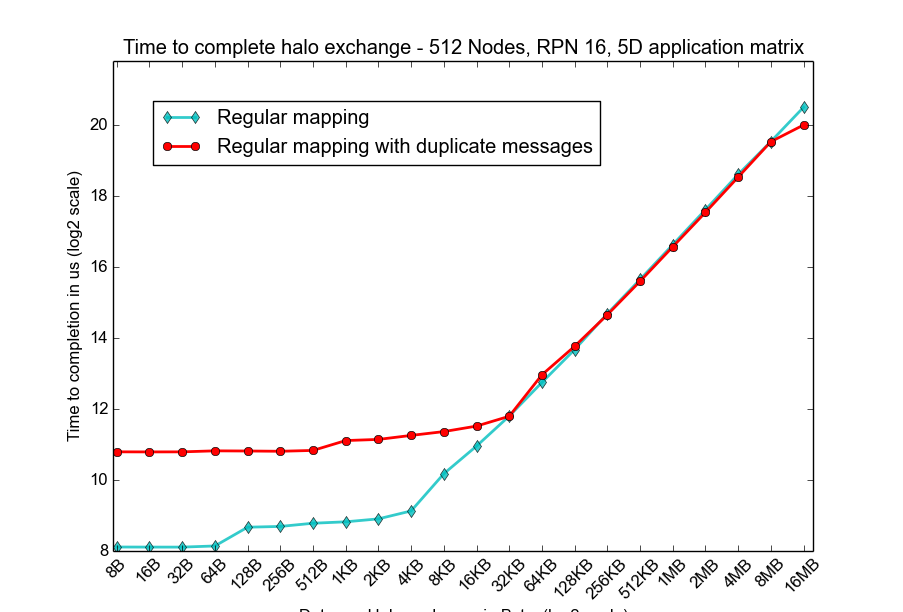
\includegraphics[width=0.475\textwidth]{regular_vs_cache_duplicates.png}
  \caption{Regular mapping with 8 duplicates and without}
    \label{fig:caching_figure_vs_without}
\end{figure}

The analytical model described in Section \ref{sect:model}, is informed by the nature of the target system
and the domain decomposition of the application. The value of a model is in the ability to predict the
results from
% What machine do we run on
%

\begin{figure}
  \center
  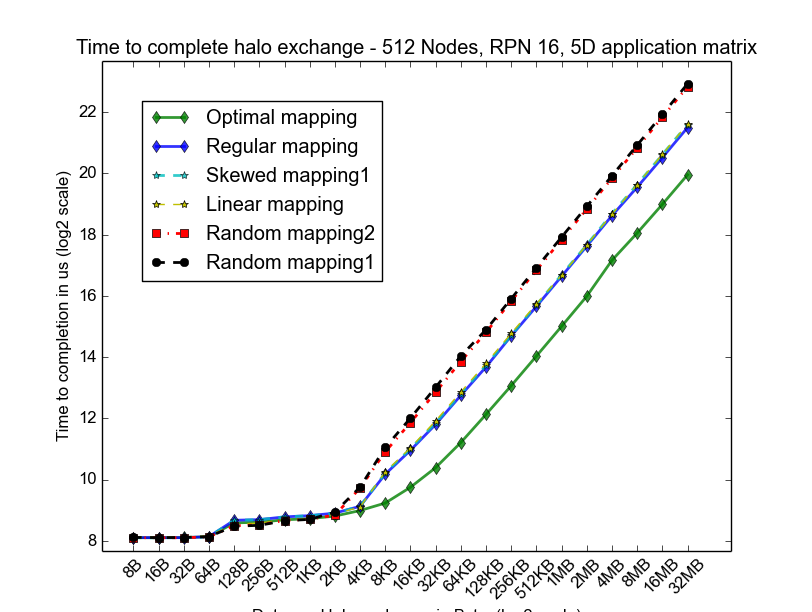
\includegraphics[width=0.475\textwidth]{5D_512_most_mappings_2.png}
  \caption{5D halo exchange on 512 nodes with 16 RPN}
    \label{fig:5D halo exchange on 512 nodes with 16 RPN}
\end{figure}


\begin{figure}
  \center
  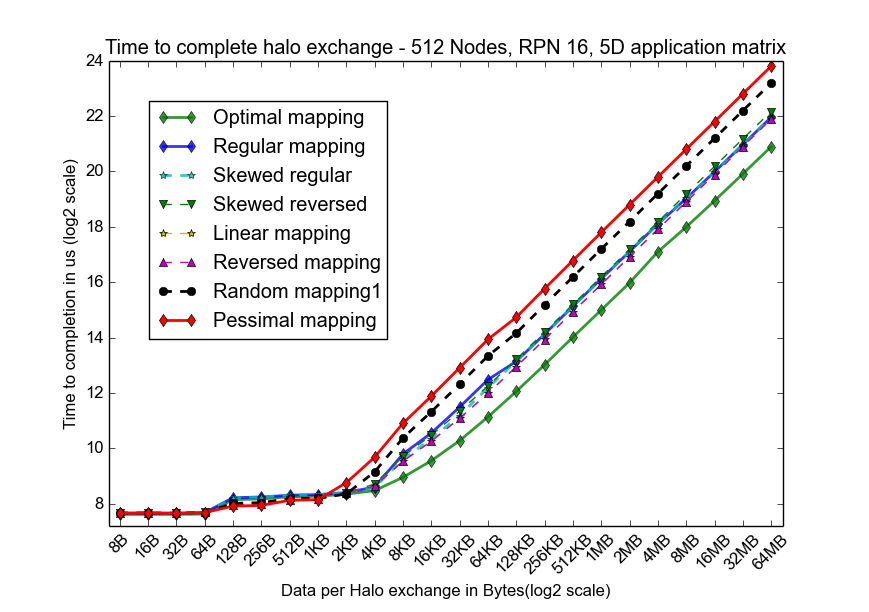
\includegraphics[width=0.51\textwidth]{3D_512_all_mappings.png}
  \caption{3D halo exchange on 512 nodes with 16 RPN}
    \label{fig:3D halo exchange on 512 nodes with 16 RPN}
\end{figure}


\section{Results}

There were three major experimental setups discussed in Section \ref{sect:experimental design}. The 

The results show that at higher data sizes, the time to completion is unaffected by the using duplicate messages of smaller size to avoid caching effects.
The plots of these two cases are shown in fig \ref{fig:caching_figure_vs_without}. From this we conclude that caching effects are negligible and can be ignored.

The plots are  \ref{fig:5D_linear_mapping}, \ref{fig:5D_optimal_mapping}, foo

\begin{figure}
  \center
  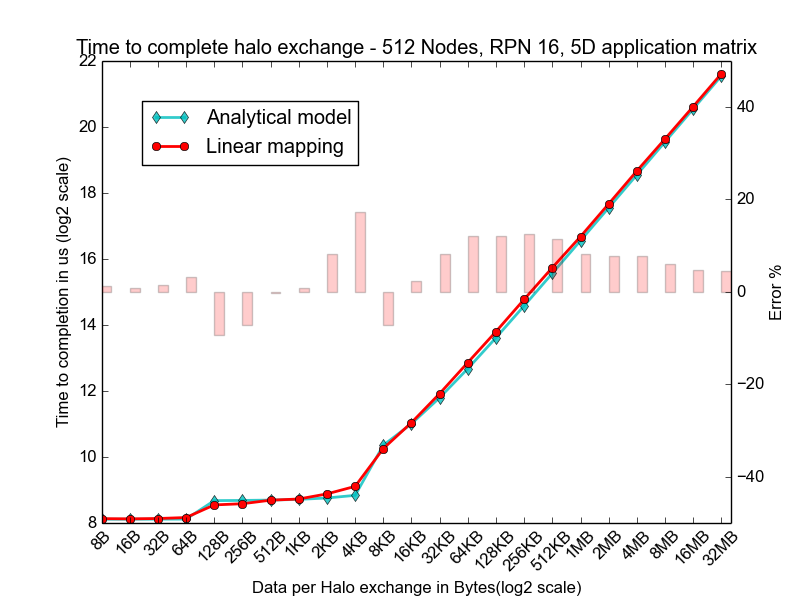
\includegraphics[width=0.45\textwidth]{mappings/5d_linear_model.png}
  \caption{Analytic model vs Experimental data for Linear mapping(5D)}
    \label{fig:5D_linear_mapping}
\end{figure}


\begin{figure}
  \center
  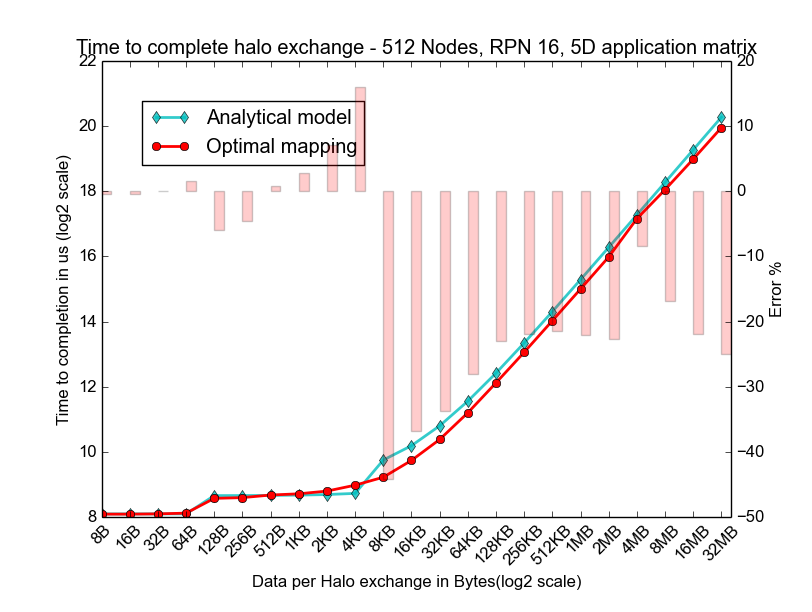
\includegraphics[width=0.45\textwidth]{mappings/5d_optimal_model.png}
  \caption{Analytic model vs Experimental data for Optimal mapping(5D)}
    \label{fig:5D_optimal_mapping}
\end{figure}

\begin{figure}
  \center
  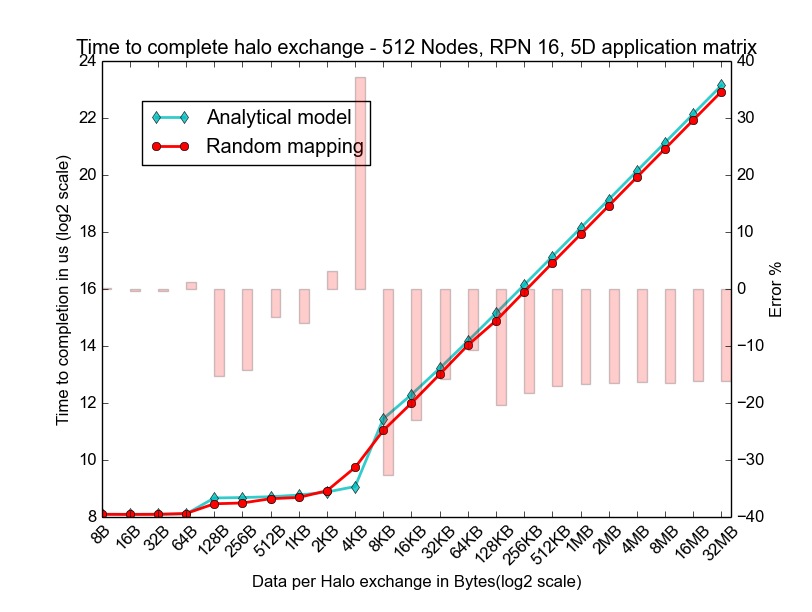
\includegraphics[width=0.45\textwidth]{mappings/5d_random_model.png}
  \caption{Analytic model vs Experimental data for Random mapping(5D)}
    \label{fig:5D_random _mapping}
\end{figure}

\begin{figure}
  \center
  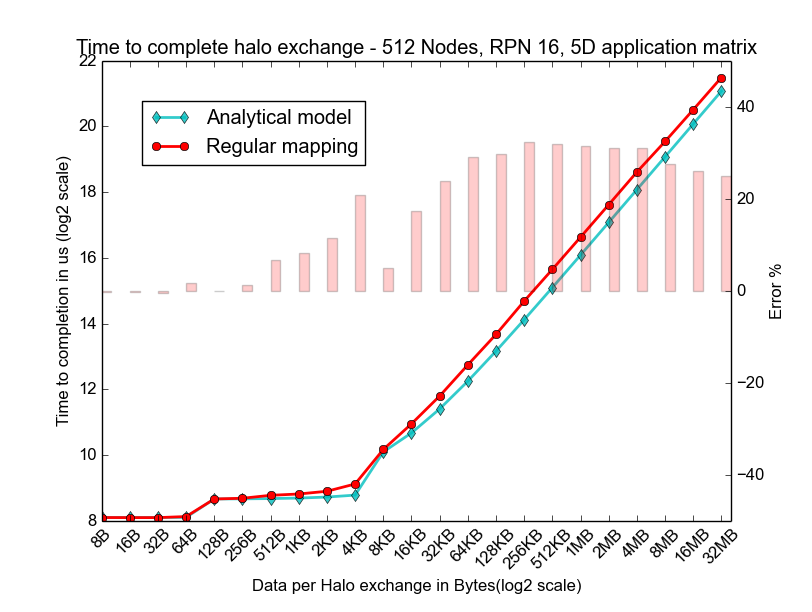
\includegraphics[width=0.45\textwidth]{mappings/5d_regular_model.png}
  \caption{Analytic model vs Experimental data for Regular mapping(5D)}
    \label{fig:5D regular mapping}
\end{figure}

\begin{figure}
  \center
  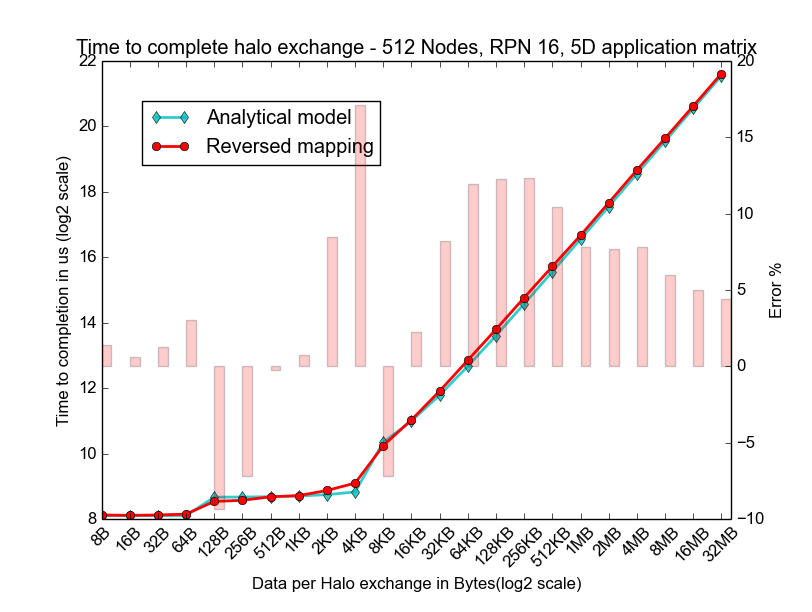
\includegraphics[width=0.45\textwidth]{mappings/5d_reversed_model.png}
  \caption{Analytic model vs Experimental data for Reversed mapping(5D)}
    \label{fig:5D_reversed_mapping}
\end{figure}

\begin{figure}
  \center
  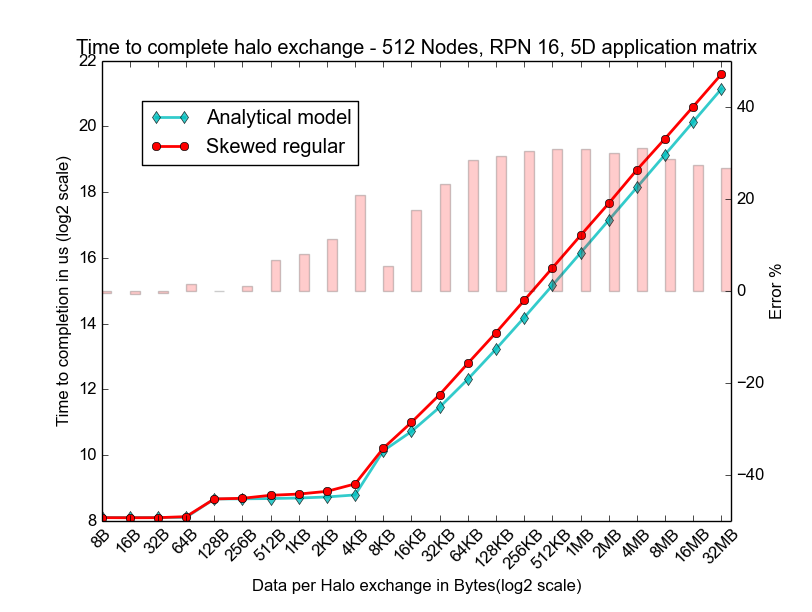
\includegraphics[width=0.45\textwidth]{mappings/5d_skewed_regular.png}
  \caption{Analytic model vs Experimental data for Skewed regular mapping(5D)}
    \label{fig:5D_skewed_regular_mapping }
\end{figure}

\begin{figure}
  \center
  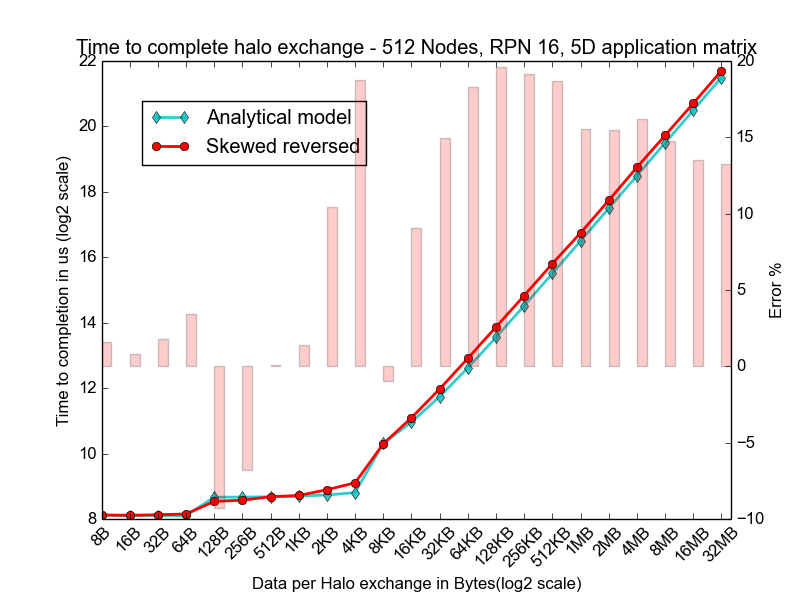
\includegraphics[width=0.45\textwidth]{mappings/5d_skewed_reversed.png}
  \caption{Analytic model vs Experimental data for Skewed reversed mapping(5D)}
    \label{fig:5D_skewed_reversed_mapping }
\end{figure}


\clearpage
\begin{figure}
  \center
  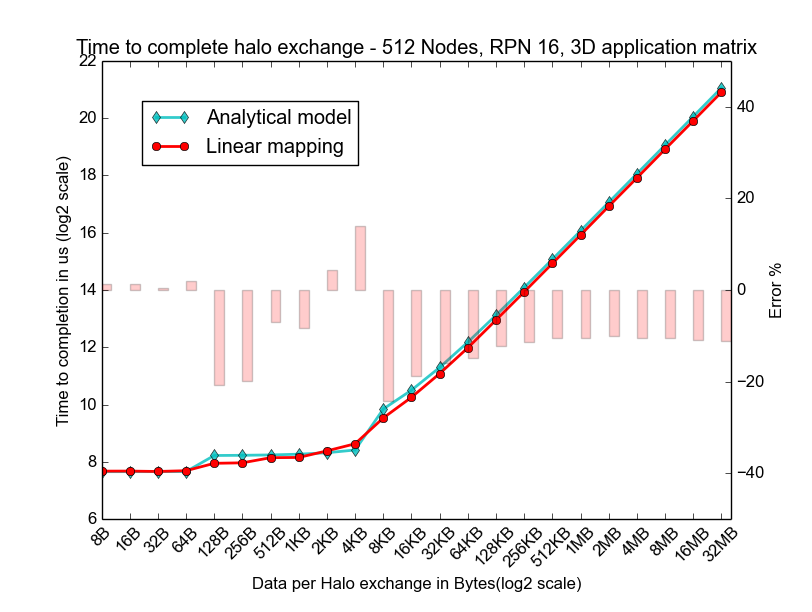
\includegraphics[width=0.45\textwidth]{mappings/3d_linear.png}
  \caption{Analytic model vs Experimental data for Linear mapping(3D)}
    \label{fig:3D_linear_mapping}
\end{figure}

\begin{figure}
  \center
  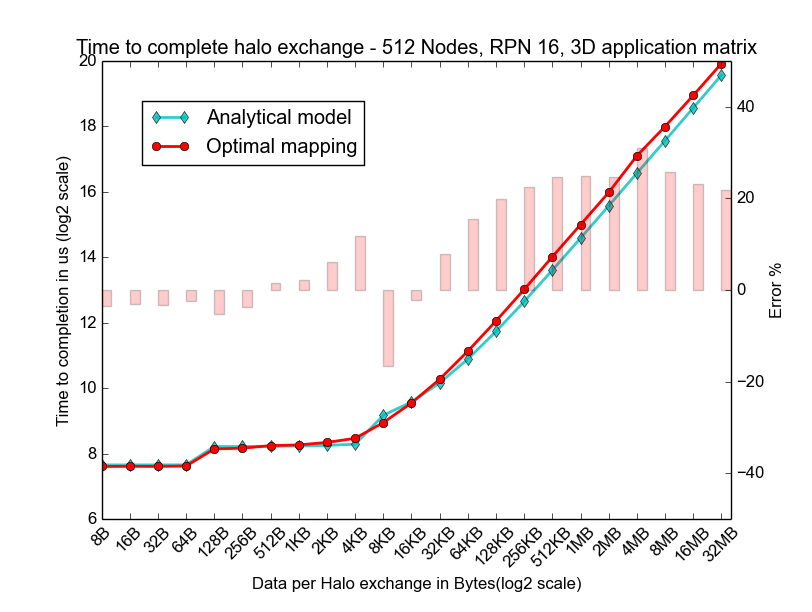
\includegraphics[width=0.45\textwidth]{mappings/3d_optimal.png}
  \caption{Analytic model vs Experimental data for Optimal mapping(3D)}
    \label{fig:3D_optimal_mapping }
\end{figure}

\begin{figure}
  \center
  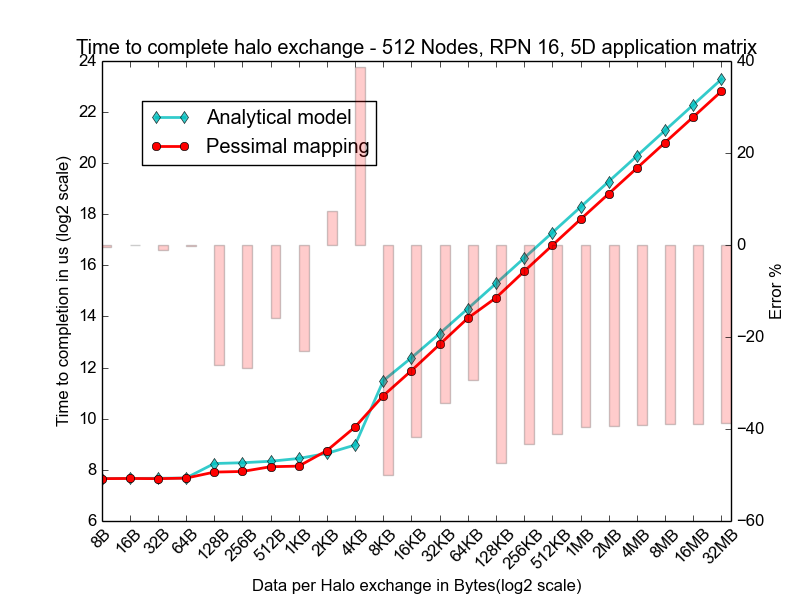
\includegraphics[width=0.45\textwidth]{mappings/3d_pessimal.png}
  \caption{Analytic model vs Experimental data for Pessimal mapping(3D)}
    \label{fig:3D_pessimal_mapping }
\end{figure}

\begin{figure}
  \center
  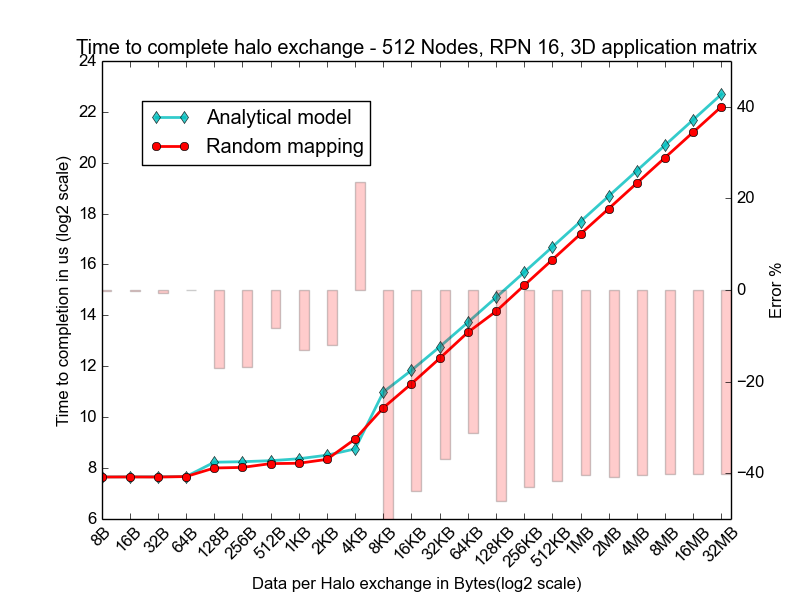
\includegraphics[width=0.45\textwidth]{mappings/3d_random.png}
  \caption{Analytic model vs Experimental data for Random mapping(3D)}
    \label{fig:3D_random_mapping }
\end{figure}

\begin{figure}
  \center
  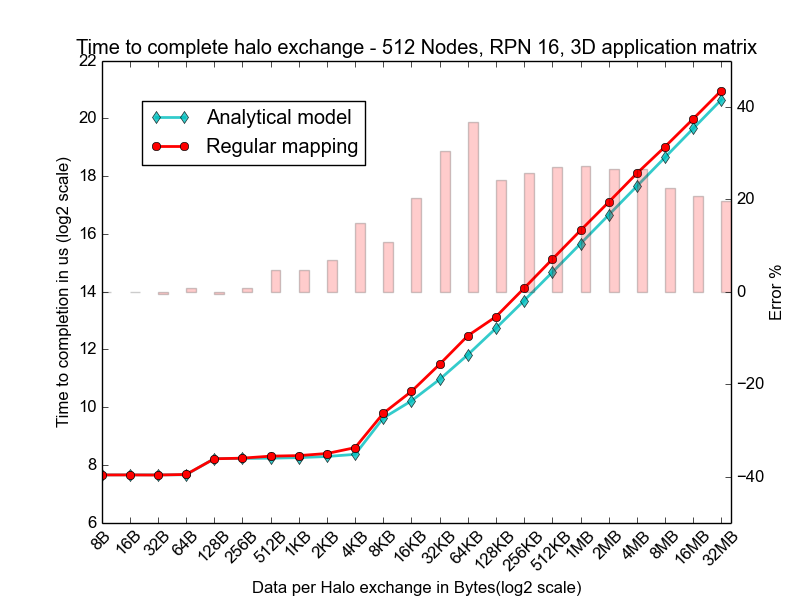
\includegraphics[width=0.45\textwidth]{mappings/3d_regular.png}
  \caption{Analytic model vs Experimental data for Regular mapping(3D)}
    \label{fig:3D_regular_mapping }
\end{figure}

\begin{figure}
  \center
  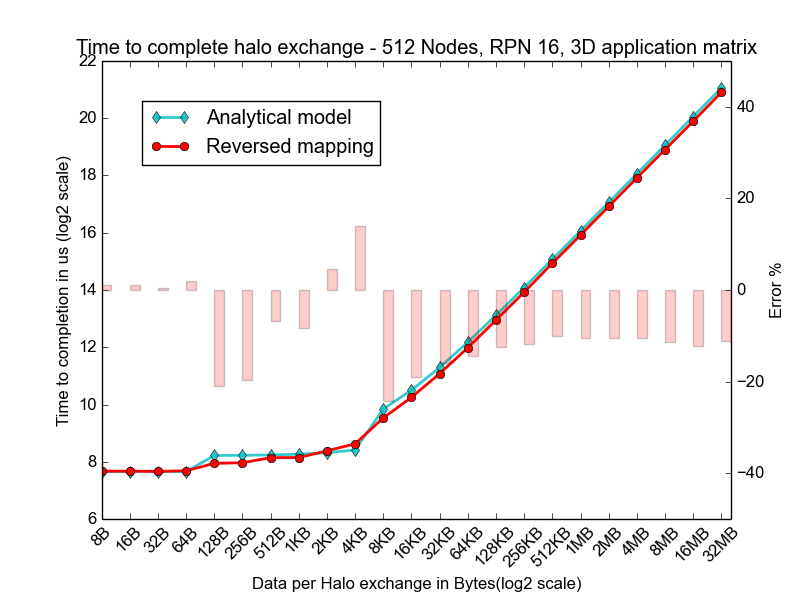
\includegraphics[width=0.45\textwidth]{mappings/3d_reversed.png}
  \caption{Analytic model vs Experimental data for Reversed mapping(3D)}
    \label{fig:3D_reversed_mapping }
\end{figure}

\begin{figure}
  \center
  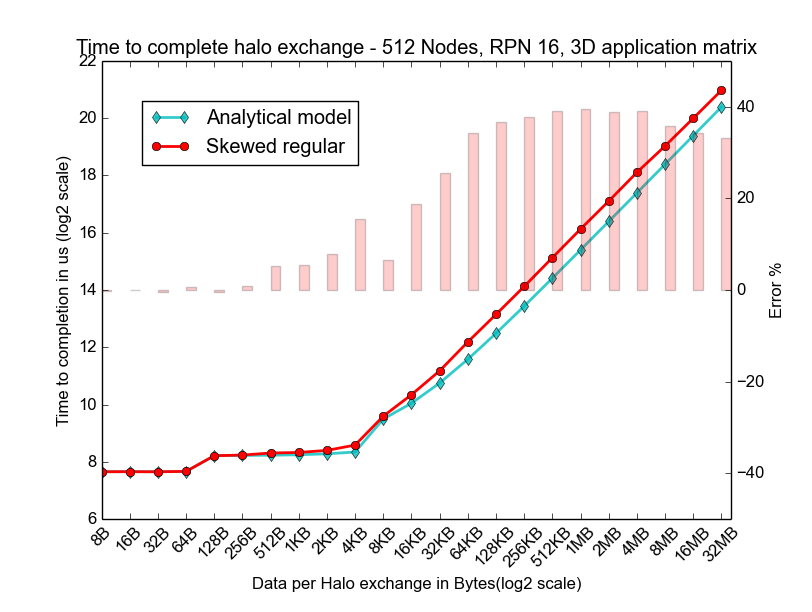
\includegraphics[width=0.45\textwidth]{mappings/3d_skewed_regular.png}
  \caption{Analytic model vs Experimental data for Skewed regular mapping(3D)}
    \label{fig:3D_skewed_regular }
\end{figure}

\begin{figure}
  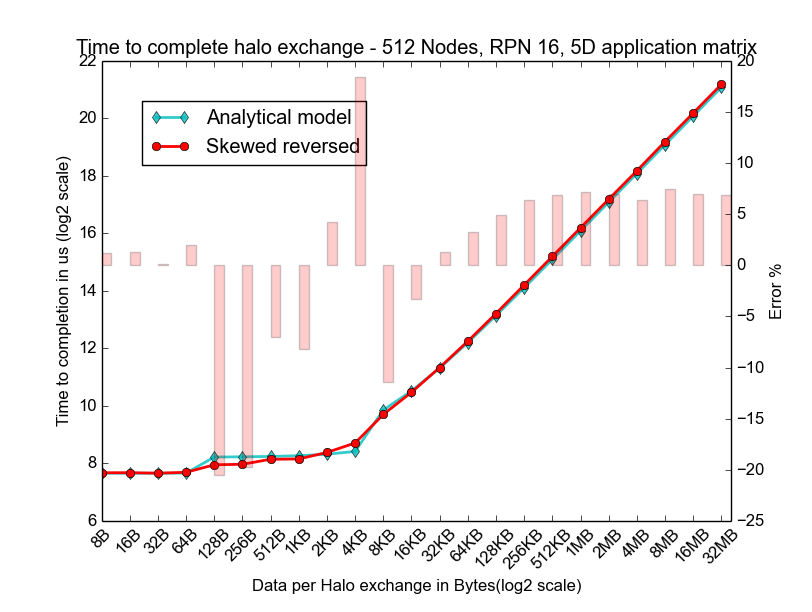
\includegraphics[width=0.45\textwidth]{mappings/3d_skewed_reversed.png}
  \caption{Analytic model vs Experimental data for Skewed reversed mapping(3D)}
    \label{fig:3D_skewed_reversed }
\end{figure}


\section{Conclusion}


\bibliographystyle{abbrv}
\bibliography{halo}

\end{document}
